\skriptsection{Spektren}{103}
\begin{minipage}{0.3\linewidth}
	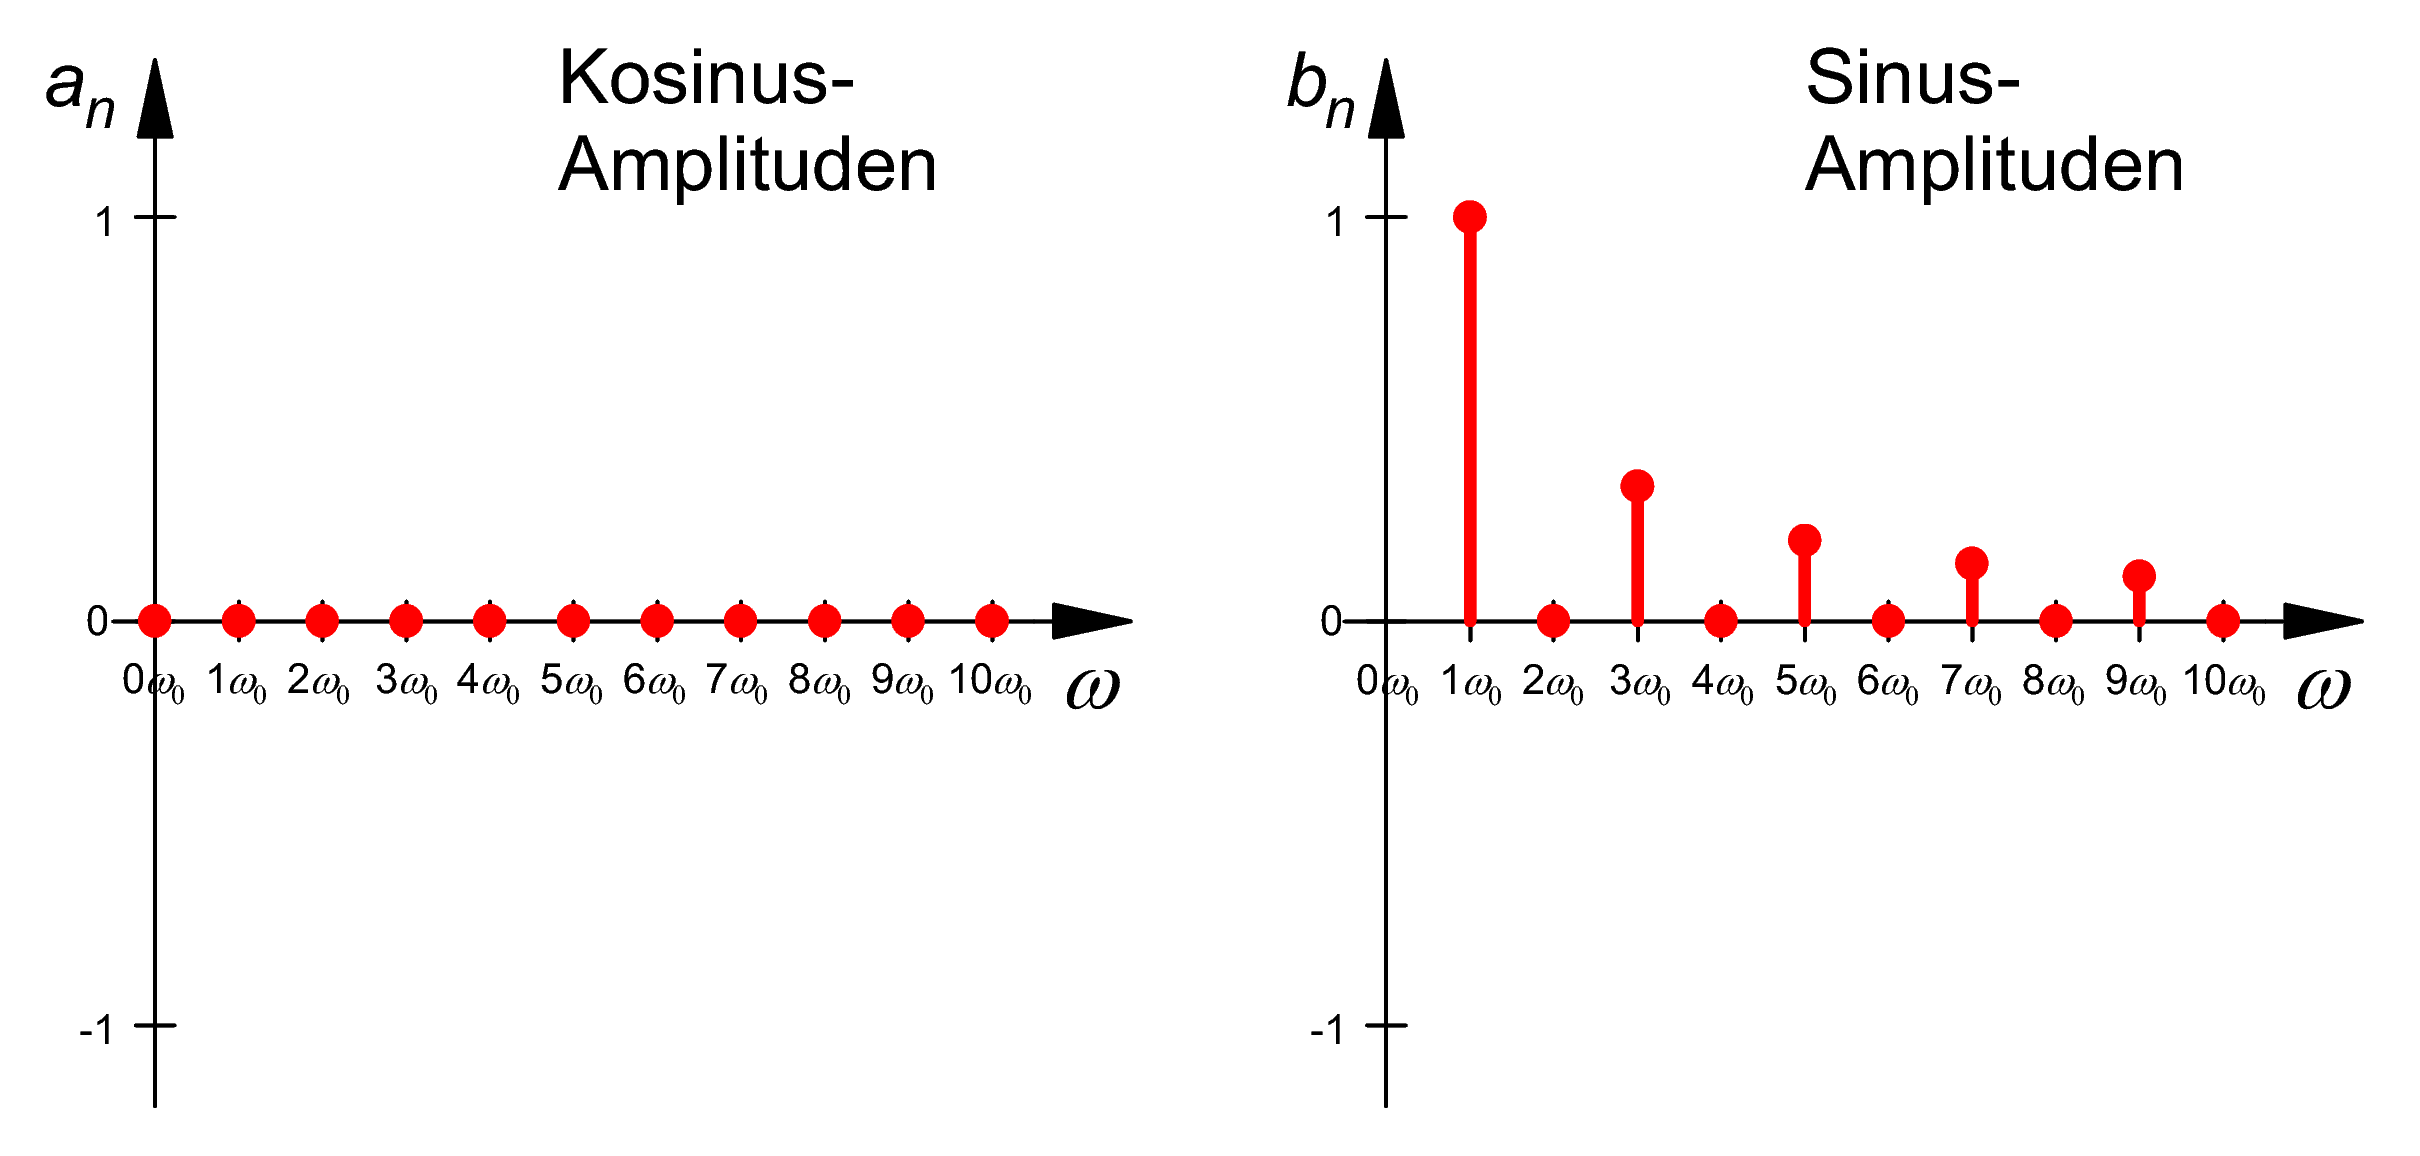
\includegraphics[width=\linewidth]{./bilder/spektren_cossin.png}
	\small{Kosinus- und Sinusamplitudendiagramm}
\end{minipage}%
\hspace{0.01\linewidth}
\begin{minipage}{0.31\linewidth}
	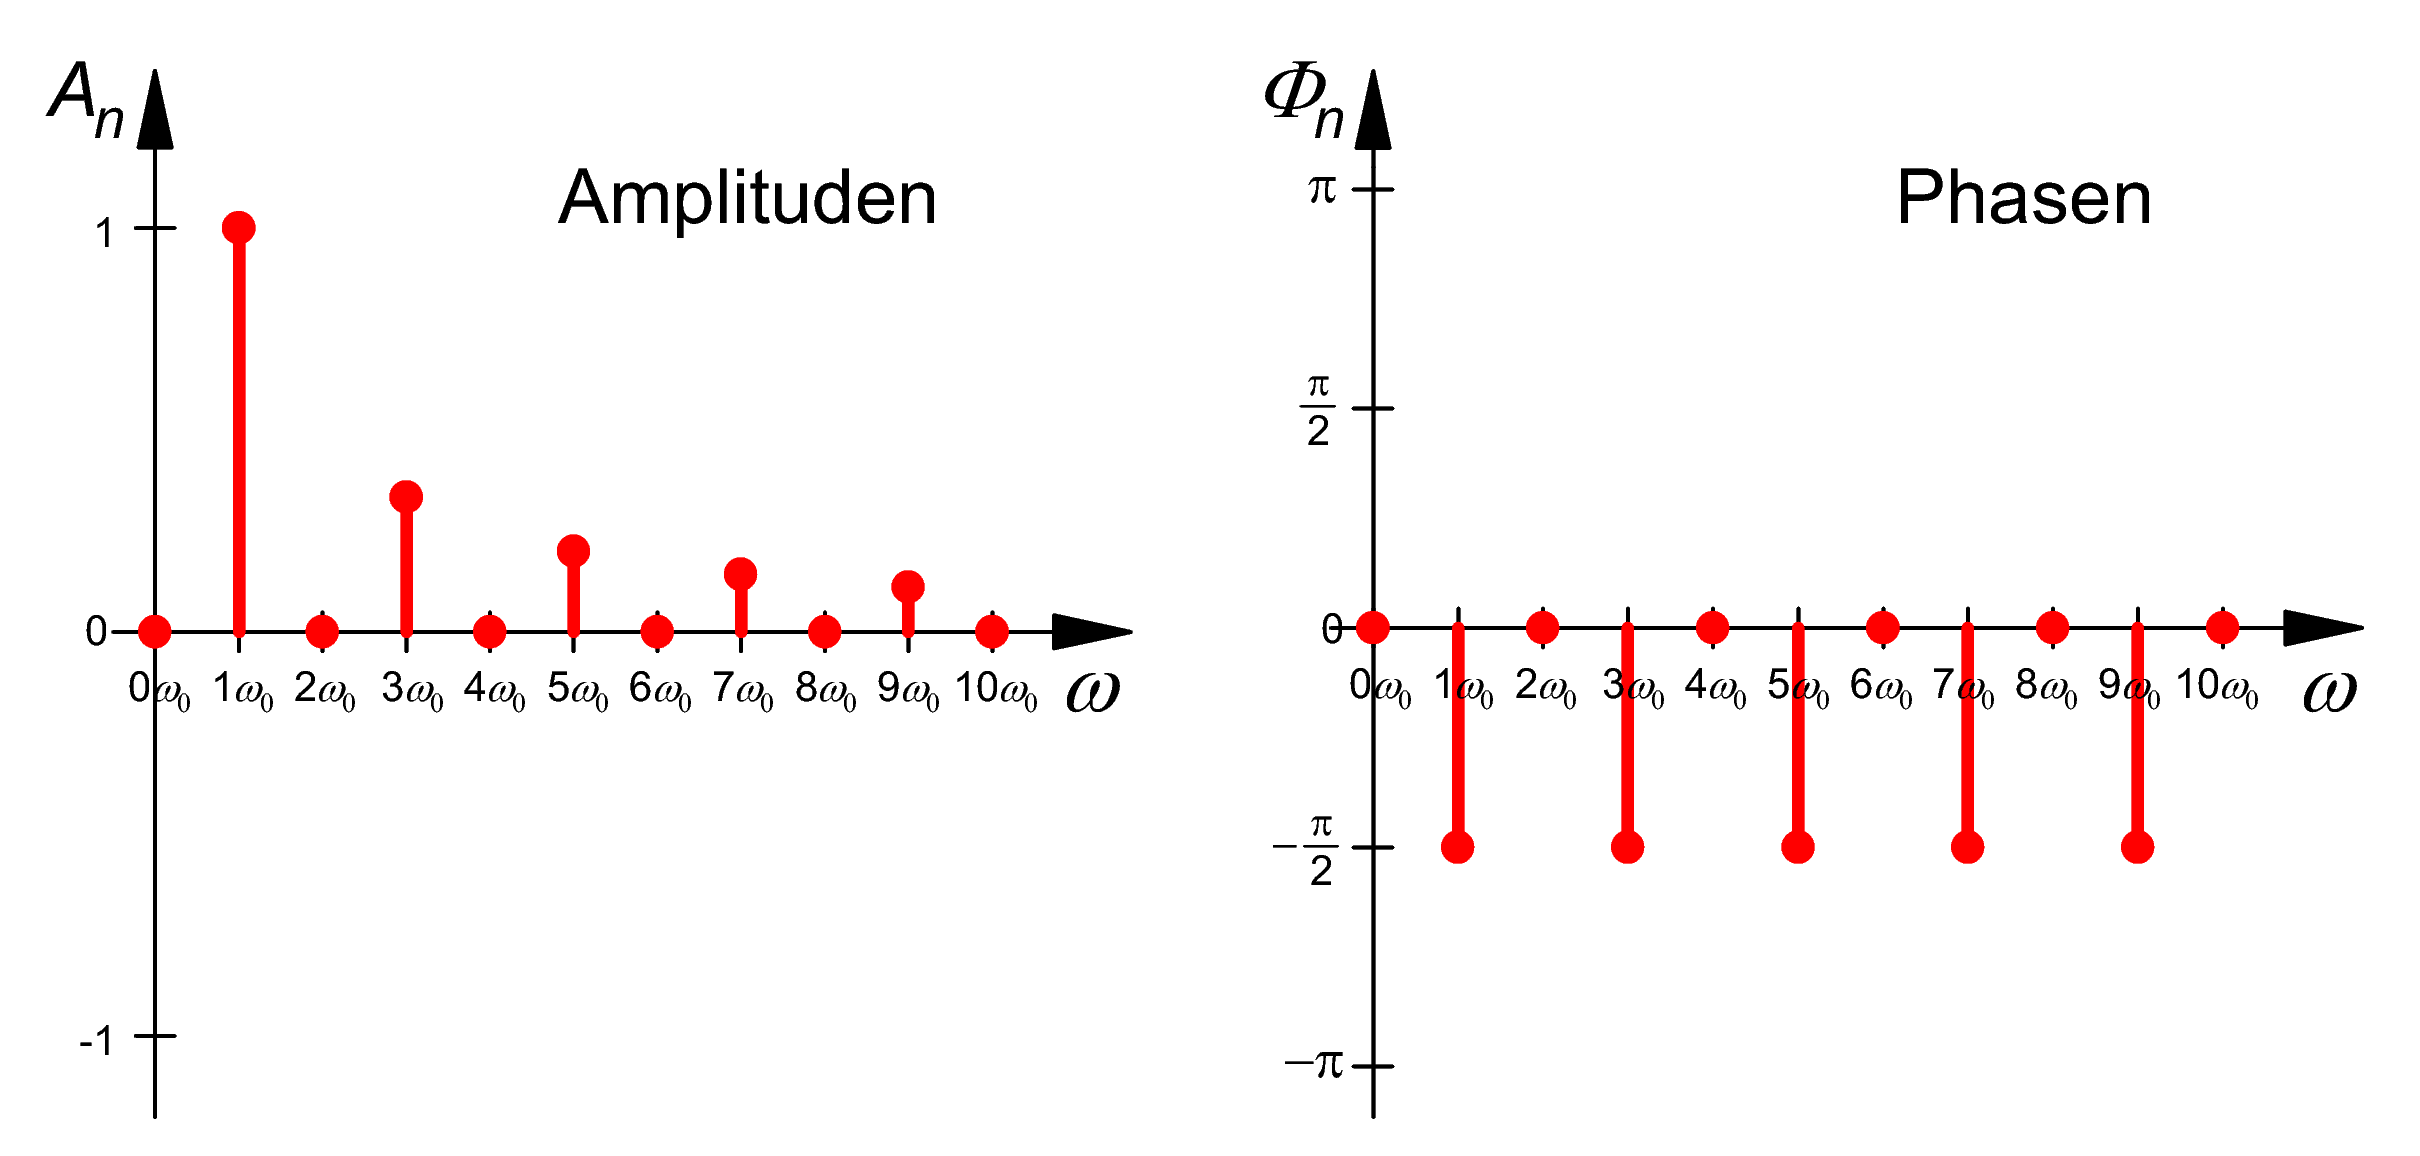
\includegraphics[width=\linewidth]{./bilder/spektren_einseitig.png}
	\small{1-seitiges Amplituden-/Phasendiagramm}
\end{minipage}%
\hspace{0.01\linewidth}
\begin{minipage}{0.31\linewidth}
	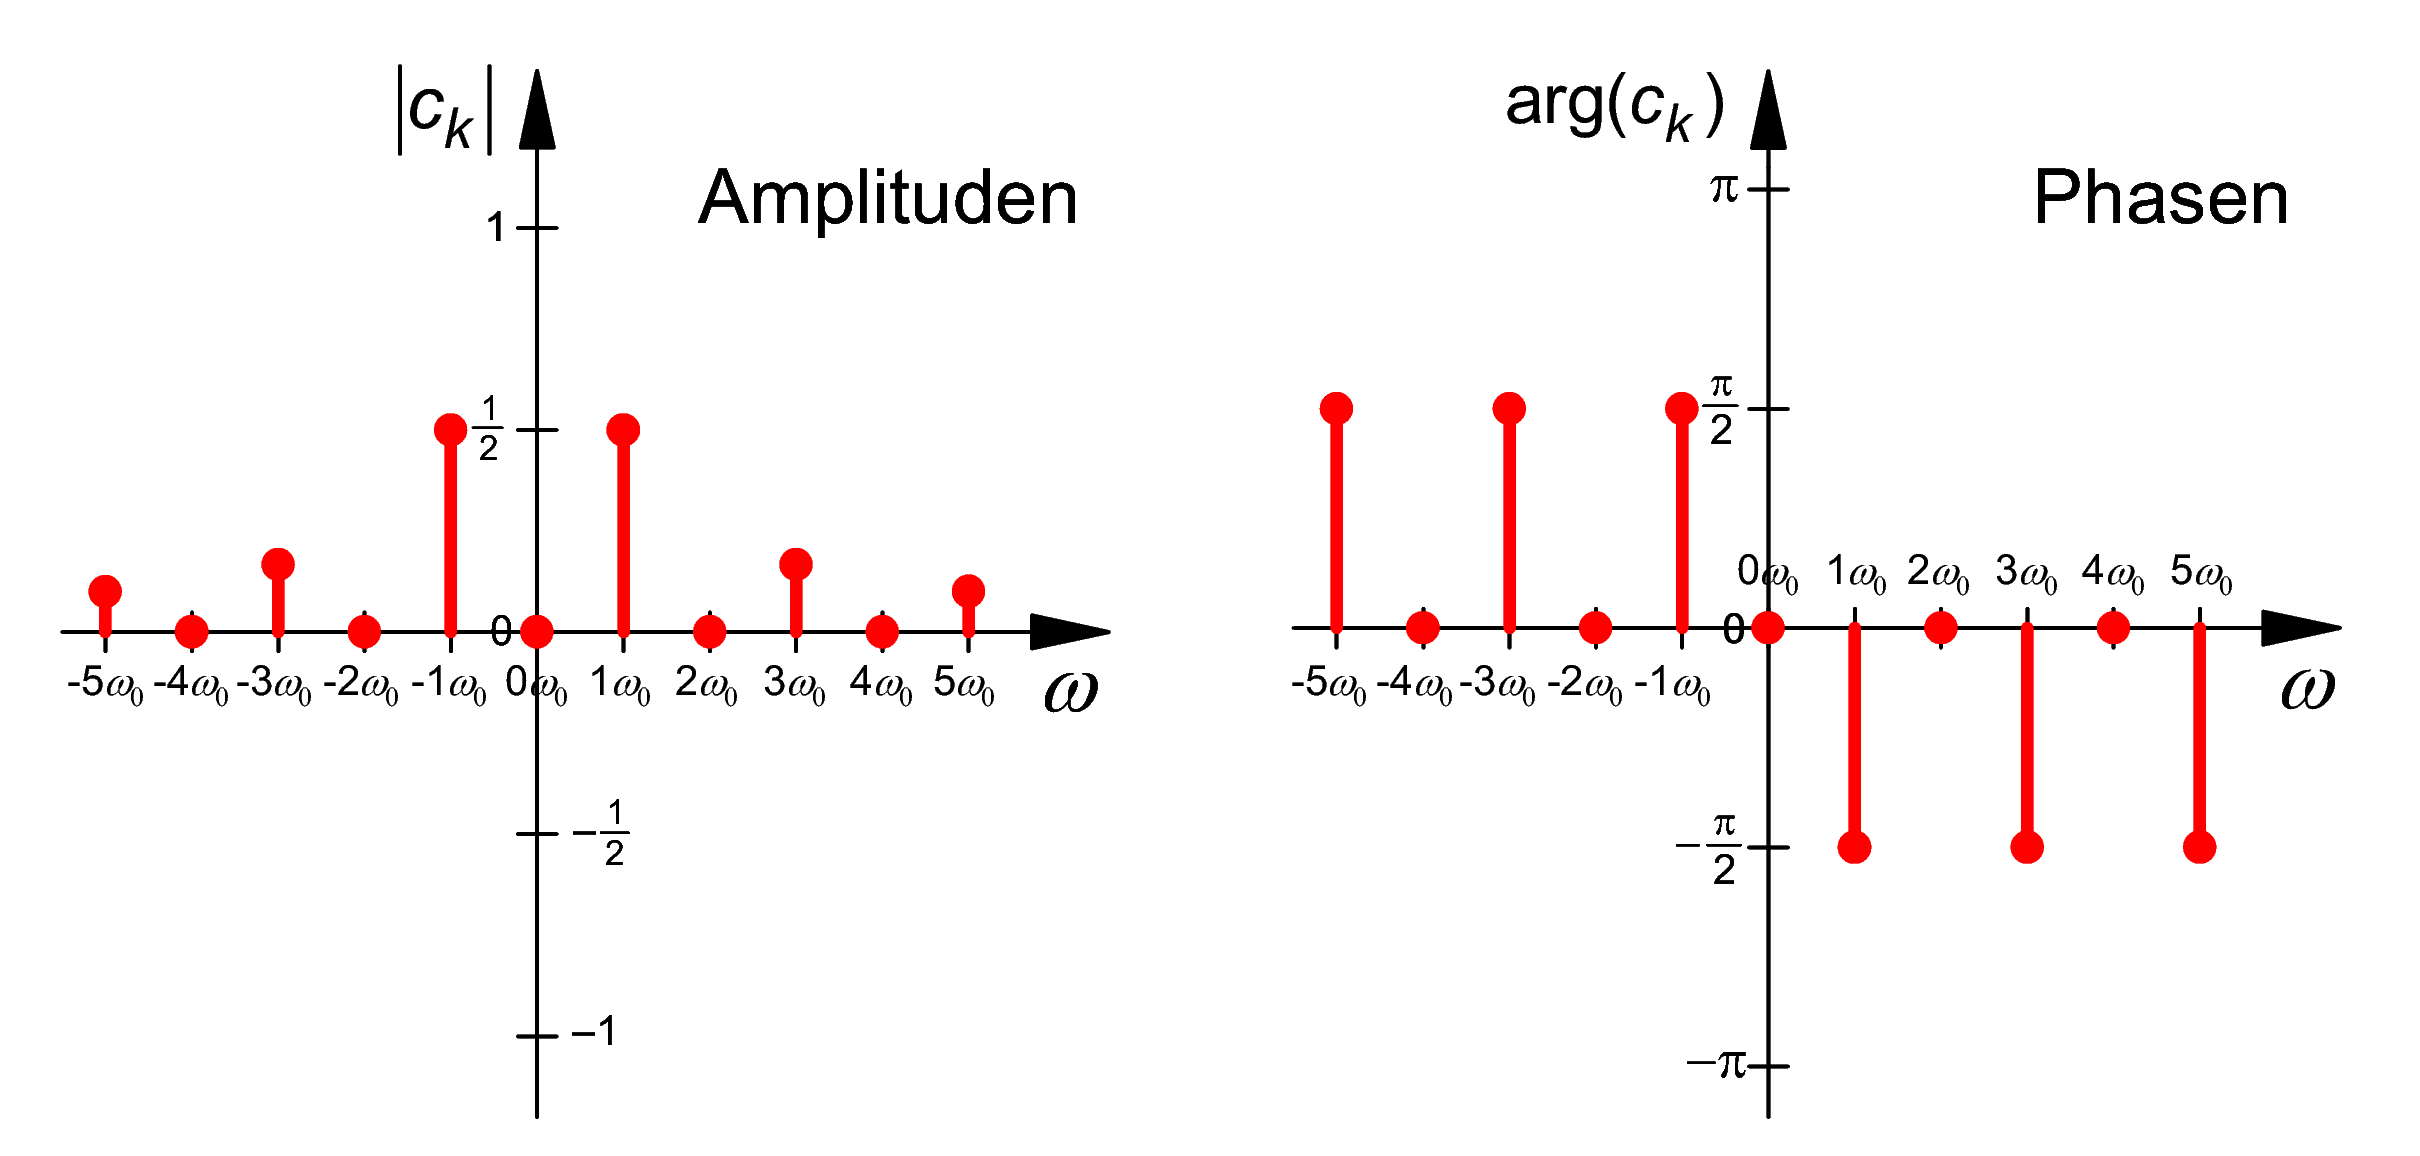
\includegraphics[width=\linewidth]{./bilder/spektren_zweiseitig.png}
	\small{2-seitiges Amplituden-/Phasendiagramm}
\end{minipage}

\subsubsection{(1) Kosinus- und Sinusamplitudendiagramm} 
Reelle Fourierkoeffizienten ($a_n, b_n$) können direkt abgelesen werden. 
Bei einer Phasenverschiebung ändern sich jedoch die Koeffizienten grafisch nicht nachvollziehbar. \\
Diese Darstellung hat gegenüber den anderen mehr Nachteile und wird daher eher selten genutzt.

$$a_n = A_n \cdot \cos(\varphi_n) = 2\cdot Re(c_n) \qquad b_n = -A_n \cdot \sin(\varphi_n) = A_n \sin(-\varphi_n) = -2\cdot Im(c_n)$$

\begin{multicols}{2}
	\subsubsection{(2) Einseitiges Amplituden-/Phasendiagramm} 
	$A_n = |a_n - j \cdot b_n| = \sqrt{a_n^2 + b_n^2}$ oder $A_n = 2 \cdot |c_n|$\\
	$\varphi_n = \arg(a_n - j \cdot b_n) = \arctan(-\frac{b_n}{a_n}) \text{ oder } \varphi_n = \arg(c_n) $ \\
	Spezialfall $n=0 \Rightarrow A_0 = |\frac{a_0}{2}| \text{ und } \varphi_0 = \left\{
	\begin{array}{l} 
	0, \quad a_0 \geq 0\\
	\pi, \quad a_0 < 0  
	\end{array}
	\right. $\\
	\vfill\null
	\columnbreak
	\subsubsection{(3) Zweiseitiges Amplituden-/Phasendiagramm}
	\textbf{(komplexes Spektrum)}\\ 
	Amplitudendiagramm ist achsensymmetrisch weil $ c_n=\overline{c_{-n}} $. Phasendiagramm ist punktsymmetrisch. \\
	Ähnlichkeit mit Einseitigem: $|c_n| = \frac{1}{2}A_n $ und $\varphi_n$ gleich wie bei (2) für alle $ n \geq 0$.\\
	$A_0 = |\frac{a_0}{2}| = |c_0| $
	$$arg(c_{-n}) = -arg(c_n) \qquad c_n = \frac{a_n - jb_n}{2} \qquad \varphi_n = arg(a_n - jb_n) \qquad c_n = \frac{A_n}{2} \cdot e^{j\varphi_n}$$
\end{multicols}

\skriptsubsection{Spezialfälle}{106}
\begin{tabular}{ll}
	Funktion f gerade 
	& (1) Sinusphasendiagramm überall 0 \\
	& (2,3) Phasendiagramm enthält nur die Werte $0$ und $\pi$ \\
	Funktion f ungerade
	& (1) Kosinusphasendiagramm überall 0 \\
	& (2,3) Phasendiagramm enthält nur die Werte $\pm \frac{\pi}{2}$ (oder $0$ falls Amplitudenwert $=0$) \\
	"Ahnlichkeit $g(t) = f(r \cdot t) $
	& (1,2,3) Das Spektrum von $g$ ist das horizontal mit den Faktor $r$ gestreckte Spektrum vom $f$. \\
	Zeitverschiebung $g(t) = f(t + t_0) $
	& (1) \verweis{Fourier_Zeitverschiebung}{Zeitverschiebung} \\
	& (2,3) Amplitudendiagramme sind identisch. \\
	& (2,3) Phasendiagramme: Die Sälule der Frequenz $k \omega_0$ wächst um $k\omega_0 t_0$. \\
	Weisses Rauschen
	& "Uberlagerung von Schwingungen aller möglichen Frequenzen \\
	& mit gleichen Amplituden und zufälligen Phasen. 
\end{tabular}
\vspace{-\baselineskip}